\documentclass[10pt]{exam}
\usepackage[phy]{template-for-exam}
\usepackage{graphicx}
\usepackage{multicol}
\usepackage{pgfplots}
\pgfplotsset{compat=1.18}


\title{Friction Lab}
\author{Rohrbach}
\date{\today}

\renewcommand{\vs}{\fillwithdottedlines{\stretch{1}}}

\begin{document}
\maketitle

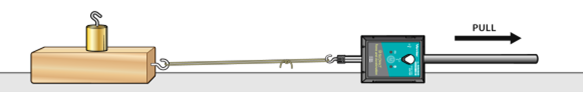
\includegraphics[scale=0.9]{friction-lab}



\begin{questions}

\uplevel{\section{Set Up}}

\question Set up your computer

\begin{parts}
  \part Using {\bf Google Chrome} (not Firefox or Safari), click the link on Schoology to launch Graphical Analysis on your computer.  
  \part Connect the sensor to your computer.
  \part Click {\bf Sensor Data Collection}.
  \part Click {\bf USB} and then {\bf LabQuest}.
  \part Make sure to Pair the LabQuest Mini, then click {\bf Done}.

  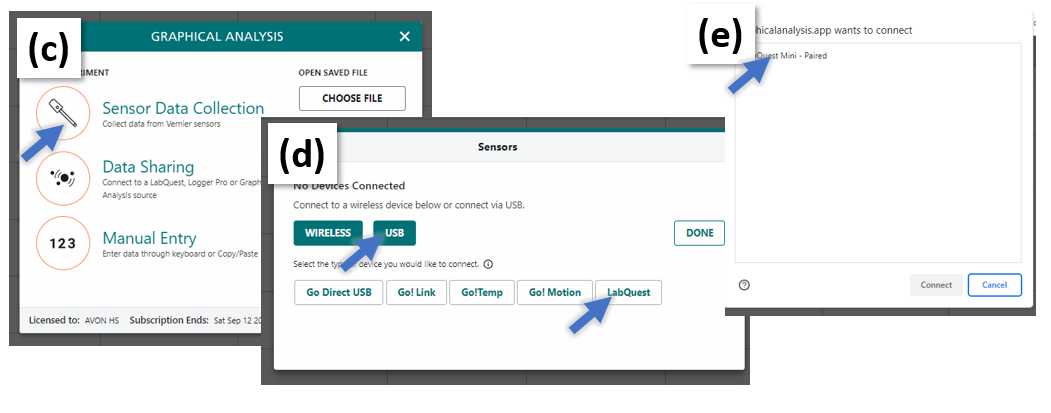
\includegraphics[width=0.75\textwidth]{ga}
\end{parts}

\question
  Make sure your Force Sensor is set to $\pm 10$ N.

\question Before you collect data, practice pulling the block and masses with the force sensor using a straight-line motion. Slowly and gently pull horizontally with a small force. \emph{Very gradually,} taking one full second, increase the force until the block starts to slide, and then keep the block moving at a constant speed for another second.


\question Zero the force sensor before collecting data.

\begin{multicols}{2}
  \begin{parts}
    \part Place the force sensor on a flat surface so the working axis is horizontal.
    \part With the force sensor axis held horizontally and no force applied, click or tap the Force meter at the bottom right of the screen and choose Zero.

    \columnbreak
    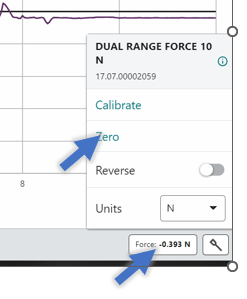
\includegraphics[width=4cm]{zero}
    
  \end{parts}
\end{multicols}

\pagebreak

\question
  Take your first set of data

  \begin{parts}
    \part   
      Stack 600 g (three 200-g weights) on top of the block.  Spread the weights evenly on the block.	
    \part
      Hold the force sensor in position, ready to pull the block, but with tension in the spring.
    \part 
      Click {\bf Collect} to start data collection. Wait a moment, then pull the block, taking care to increase the force gradually.
    \part
      Inspect your graph. It should reflect the desired motion, including pulling the block at constant speed once it begins moving. If it does not, start data collection and repeat the pulling process. Sketch the graph below for reference

      \begin{tikzpicture}
        \begin{axis}[
          xlabel={\bf time},
          ylabel={\bf force},
          ymin=-5,
          ymax=5,
          xmin=0,
          xmax=4,
          ytick=\empty,
          xtick=\empty,
          axis y line = left,
          axis x line = center,
          height = 6cm,
          width = 15cm
        ]
        \end{axis}
      \end{tikzpicture}
    
  \end{parts}




\question
  Explain what your graph shows.  Is static friction greater or less than kinetic friction?  Why might this make sense at the microscopic level?
  \fillwithdottedlines{15em}
  

\begin{EnvUplevel}
  \section{Static Friction and Kinetic Friction}

  In this part, you will measure the peak static friction force and the kinetic friction force as a function of the normal force on the block. In each run, you will pull the block as before, but by changing the masses on the block, you will vary the normal force on the block. 
\end{EnvUplevel}

\question 
  Remove all masses from the block.
\question
	Using the same procedure as before, collect force vs. time data.
\question
  Click the graph to examine the data. The maximum value of the force occurs when the block started to slide. Click or tap the peak static friction force and record the value in your data table. \emph{Note: You can also adjust the Examine line by dragging the line.}

\pagebreak

\question
  Next you need to determine the average friction force while the block was moving at constant velocity.

  \begin{multicols}{2}

    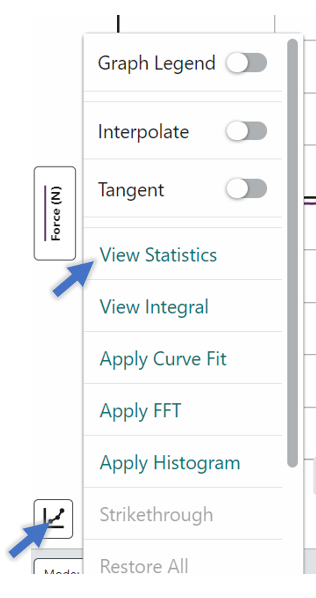
\includegraphics[width=4cm]{graph-tools}
    \begin{parts}
      \part 
        Select the data in the approximately constant-force region of the graph.
      \part
        Find the `Graph Tools' Icon at the bottom left of the screen then click {\bf View Statistics}.
      \part
        Record the mean force value in your data table.
    \end{parts}

  \end{multicols}

\question
  Repeat Steps 10-12 for two more measurements and average the results to determine the reliability of your measurements. Record the values in the data table. 
\question
  Repeat steps 10-13 for the block with 200 g, 400 g, and 600 g added on top.

  \begin{tabular}{|l
    *3{|>{\centering\arraybackslash}m{.15\textwidth}}
    ||>{\centering\arraybackslash}m{.15\textwidth}|}
    \hline
    & \multicolumn{4}{c|}
    {\bf Maximum Static Friction (N)}  \\\cline{2-5}
    & \center Trial 1 &
     \center Trial 2 & 
     \center Trial 3 &   Average 
     \\[0.5em]\hline\hline
    block &&&&\\[2em]\hline
    block + 200 g &&&&\\[2em]\hline
    block + 400 g &&&&\\[2em]\hline
    block + 600 g &&&&\\[2em]\hline
  \end{tabular}

  \begin{tabular}{|l
    *3{|>{\centering\arraybackslash}m{.15\textwidth}}
    ||>{\centering\arraybackslash}m{.15\textwidth}|}
    \hline
    & \multicolumn{4}{c|}
    {\bf Average Kinetic Friction (N)}  \\\cline{2-5}
    & \center Trial 1 &
     \center Trial 2 & 
     \center Trial 3 &   Average 
     \\[0.5em]\hline\hline
    block &&&&\\[2em]\hline
    block + 200 g &&&&\\[2em]\hline
    block + 400 g &&&&\\[2em]\hline
    block + 600 g &&&&\\[2em]\hline
  \end{tabular}


\question
  How does the weight added to the block affect its friction?  Why does this make sense at a microscopic level?
  \vs

\question
  What do you think would happen if we turned the block on its side so that the surface area that was touching the table was smaller?
  \vs

\question
  What do you think would happen if we turned the block over and did the same experiment with the rubber side down?
  \vs


\begin{EnvUplevel}
  \section{Conclusions}
\end{EnvUplevel}

\question 
  What factors affect the amount of friction that act on an object?
  \vs

\pagebreak

\vfill
  
\end{questions}



\end{document}